\subsection{Arsitektur Dasar Acuan (RADAR)}

RADAR akan menjadi dasar acuan yang digunakan sebagai dasar perbandingan kinerja. Arsitektur ini terdiri atas dua komponen, yaitu komponen layanan tiket dan kluster PostgreSQL. Kluster PostgreSQL ini terdiri atas satu \textit{leader} dan beberapa replika. Penggunaan replika bertujuan untuk meningkatkan \textit{throughput} pada operasi baca.

\begin{figure}[htbp]
    \centering
    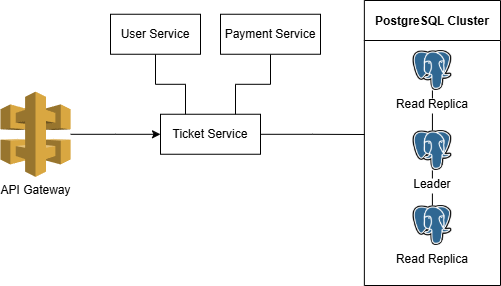
\includegraphics[width=0.8\textwidth]{resources/appendix/architecture-reference.png}
    \caption{Arsitektur Dasar Acuan}
    \label{fig:baseline-architecture}
\end{figure}

\subsubsection{Isu \textit{Replication Lag}}

Salah isu yang perlu diperhatikan pada arsitektur ini adalah \textit{replication lag}. Replika yang tertinggal selama beberapa detik pada kasus ini akan berdampak signifikan. Pada kasus ini, pendekatan solusinya akan bergantung pada keadaan yang dihadapi selama implementasi.

Pada proses pengujian, kluster PostgreSQL ini akan ditempatkan pada satu \textit{availability zone} yang sama, sehingga \textit{replication lag} tidak akan terjadi secara signifikan. Meskipun begitu, apabila terjadi \textit{replication lag} yang sangat besar, alternatif solusinya adalah dengan mengharuskan replika ACK terlebih dahulu sebelum penulisan dapat dilakukan, alih-alih melakukan replikasi secara asinkron.

\subsubsection{Penskalaan Pada RADAR}

Komponen \textit{backend} utama (layanan tiket) bersifat \textit{stateless}, sehingga dapat di-\textit{scale} dengan meningkatkan jumlah \textit{instance}. Kemudian, gerbang API akan melakukan \textit{load balancing} untuk mendistribusikan beban ke beberapa \textit{instance}.

Basis data merupakan komponen yang sulit di-\textit{scale} secara dinamis berdasarkan beban yang diterima. Biasanya, penskalaan secara vertikal merupakan opsi utama untuk meningkatkan \textit{throughput}, terutama dalam operasi tulis. Arsitektur ini membuat kluster PostgreSQL dengan konfigurasi satu node pemimpin dan sisanya node replika. Keberadaan replika memungkinkan peningkatan \textit{throughput} permintaan baca, meski tidak ada peningkatan \textit{throughput} untuk operasi tulis.

\subsubsection{Aspek Lain}

Pada saat penjualan, dapat diasumsikan entitas Events, TicketCategory, Areas, TicketSale, dan TicketPackage tidak berubah sehingga data entitas tersebut dapat di-\textit{cache}.